% Supp Fig. (error-budget flowchart): master decomposition of the discretization error.
% Standalone TikZ source; compile with pdflatex -> ../figure9.pdf
% Explicit coordinates throughout (no relative-positioning surprises).
\documentclass[border=3pt]{standalone}
\usepackage{amssymb,amsmath}
\usepackage{tikz}
\usetikzlibrary{arrows.meta,calc}
\definecolor{banana}{HTML}{FFD932}
\definecolor{cgblue}{HTML}{007CA5}
\definecolor{isabelline}{HTML}{EAEDEA}
\begin{document}
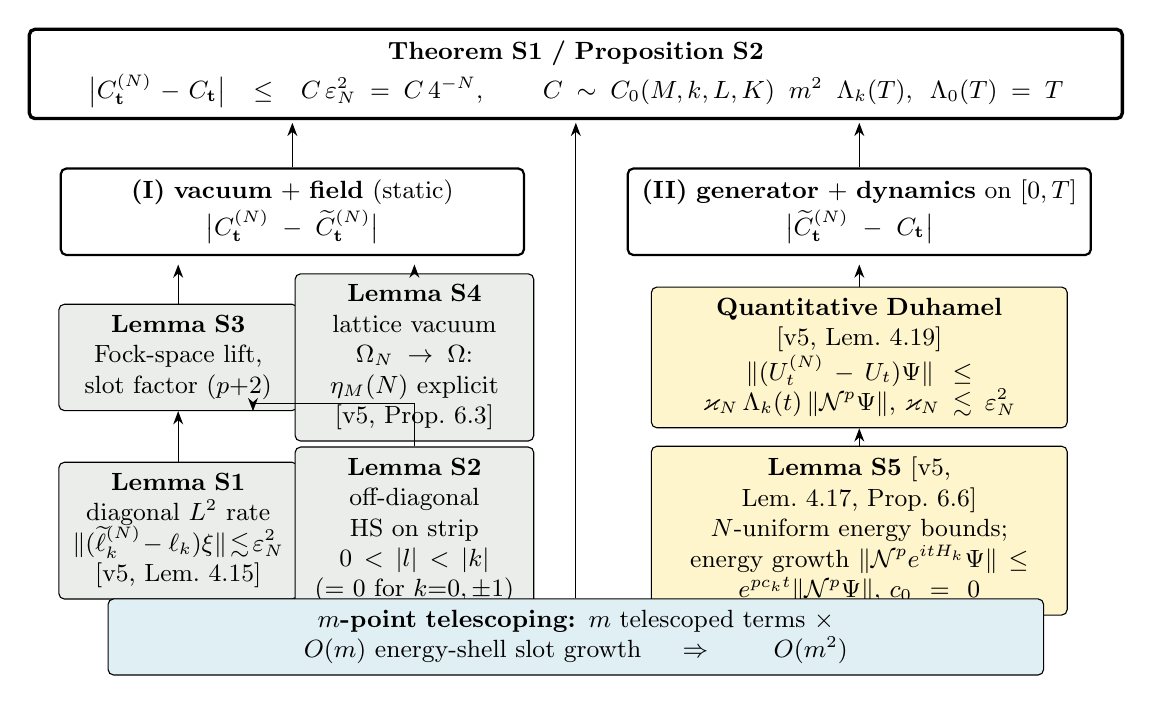
\begin{tikzpicture}[>=Stealth, font=\small,
  box/.style={draw, rounded corners=2pt, align=center, inner sep=4pt},
  leaf/.style={box, fill=isabelline, text width=2.75cm},
  leafdyn/.style={box, fill=banana!25, text width=5.0cm},
  branch/.style={box, thick, fill=white, text width=5.6cm},
  root/.style={box, very thick, fill=white, text width=13.6cm}]

  % ---- root: Theorem S1 ----
  \node[root] (root) at (0,0)
    {\textbf{Theorem S1 / Proposition S2}\\[2pt]
     $\bigl|C^{(N)}_{\mathbf t}-C_{\mathbf t}\bigr|\;\le\;C\,\varepsilon_{N}^{2}=C\,4^{-N}$,
     \qquad $C\sim C_{0}(M,k,L,K)\; m^{2}\; \Lambda_{k}(T)$, \ $\Lambda_{0}(T)=T$};

  % ---- level 2: the two terms of the master decomposition (Prop. S1) ----
  \node[branch] (static) at (-3.6,-1.75)
    {\textbf{(I) vacuum $+$ field} (static)\\[1pt]
     $\bigl|C^{(N)}_{\mathbf t}-\widetilde C^{(N)}_{\mathbf t}\bigr|$};
  \node[branch] (dyn) at (3.6,-1.75)
    {\textbf{(II) generator $+$ dynamics} on $[0,T]$\\[1pt]
     $\bigl|\widetilde C^{(N)}_{\mathbf t}-C_{\mathbf t}\bigr|$};

  \draw[->] (static.north) -- (-3.6,-0.62);
  \draw[->] (dyn.north) -- (3.6,-0.62);

  % ---- static column: S1,S2 feed the Fock lift S3; S4 is the vacuum input ----
  \node[leaf] (s3) at (-5.05,-3.60)
    {\textbf{Lemma S3}\\ Fock-space lift,\\ slot factor $(p{+}2)$};
  \node[leaf] (s4) at (-2.05,-3.60)
    {\textbf{Lemma S4}\\ lattice vacuum $\Omega_{N}\to\Omega$:\\ $\eta_{M}(N)$ explicit [v5, Prop.\ 6.3]};
  \node[leaf] (s1) at (-5.05,-5.80)
    {\textbf{Lemma S1}\\ diagonal $L^{2}$ rate\\ $\lVert(\widetilde\ell^{(N)}_{k}\!-\ell_{k})\xi\rVert\!\lesssim\!\varepsilon_{N}^{2}$ [v5, Lem.\ 4.15]};
  \node[leaf] (s2) at (-2.05,-5.80)
    {\textbf{Lemma S2}\\ off-diagonal HS on strip\\ $0<|l|<|k|$ ($=0$ for $k{=}0,\pm1$)};

  \draw[->] (s3.north) -- (-5.05,-2.42);
  \draw[->] (s4.north) -- (-2.05,-2.42);
  \draw[->] (s1.north) -- (s3.south);
  \draw[->] (s2.north) -- ++(0,0.55) -| ($ (s3.south)+(0.95,0) $);

  % ---- dynamics column: S5 (energy bounds) feeds the Duhamel bound ----
  \node[leafdyn] (duh) at (3.6,-3.60)
    {\textbf{Quantitative Duhamel} [v5, Lem.\ 4.19]\\
     $\lVert(U^{(N)}_{t}-U_{t})\Psi\rVert\le\varkappa_{N}\,\Lambda_{k}(t)\,\lVert\mathcal N^{p}\Psi\rVert$, $\varkappa_{N}\lesssim\varepsilon_{N}^{2}$};
  \node[leafdyn] (s5) at (3.6,-5.80)
    {\textbf{Lemma S5} [v5, Lem.\ 4.17, Prop.\ 6.6]\\ $N$-uniform energy bounds;\\
     energy growth $\lVert\mathcal N^{p}e^{itH_{k}}\Psi\rVert\le e^{p c_{k}t}\lVert\mathcal N^{p}\Psi\rVert$, $c_{0}=0$};

  \draw[->] (duh.north) -- (3.6,-2.42);
  \draw[->] (s5.north) -- (duh.south);

  % ---- bottom: telescoping (feeds the m^2 in the constant) ----
  \node[box, fill=cgblue!12, text width=11.6cm] (tel) at (0,-7.15)
    {\textbf{$m$-point telescoping:} $m$ telescoped terms $\times$ $O(m)$
     energy-shell slot growth $\;\Rightarrow\; O(m^{2})$};
  \draw[->] (tel.north) -- (0,-0.62);

\end{tikzpicture}
\end{document}
